\chapter{Relevant Theoretical Issues \label{sec:theory}}

\section{Introduction}
Our understanding of particles and how they interact is constantly evolving through new experimental results and theoretical breakthroughs.
In this chapter, the current theoretical framework in particle physics and theories of physics beyond this framework are briefly described.
The discussion is focused towards the theoretical background for searches for new long-lived charged particles with the Compact Muon Solenoid (CMS) experiment
at the Large Hadron Collider (LHC) (see Ch.~\ref{sec:app}).

\section{Standard Model \label{sec:SM}}
The standard model (SM) of particle physics is a framework for describing fundamental and composite particles and the forces that govern how they interact. 
A summary of the SM is given below, more information can be found in~\cite{griffiths2008introduction, Srednicki_2007}.

Particles in the SM are split into two types: bosons, which have integer spin, and fermions, which have half integer spin.
The bosons, except for the Higgs Boson, are the carriers of the forces of the SM while the fermions act as the matter fields.
The Higgs Boson has a special role discussed below.

%The forces in the SM are the electromagnetic, strong, and weak forces. The carrier of the strong force is the 

Formally, the SM is described according to the symmetry group
\begin{equation}
SU(3)_C \times SU(2)_L \times U(1)_Y
\label{eq:SMGroups}
\end{equation}
where SU(N) denotes special unitary groups of dimension N. 
%Special unitary groups have the property of having a determinant of one.
Reading from left to right the groups represent color, weak isospin, and hypercharge. 
The color symmetry group is responsible for the strong force which is carried by the gluon.
A mixture of the weak isospin and hypercharge groups are responsible for the weak and electromagnetic forces. Left-handed fermions are doublets of the
isospin group while the right handed fermions are singlets as they do not interact with the raising and lowering operators of the SU(2) group.
The weak force is carried by the $W$ and $Z$ bosons while the electromagnetic force is carried by the photon.

The last of the bosons in the SM to be discovered is the Higgs Boson. The Higgs Boson is a scalar which allows it to have a non-zero vacuum expectation value 
(VEV)~\cite{PhysRevLett.13.508, PhysRevLett.13.321}.
This non-zero VEV breaks the electroweak symmetry and results in the $W$ and $Z$ bosons acquiring mass while the photon remains massless.
The Higgs Boson's non-zero VEV also gives mass to the fermions by allowing for a coupling between the singlet right handed fermions and doublet left handed fermions
which is otherwise not allowed.
%Describe the Higgs mechanism in this paragraph, don't really know how to do it currently.
In July 2012, the CMS and ATLAS experiments at the LHC
announced the discovery of a new particle with properties similar to the Higgs Boson~\cite{Chatrchyan:2012ufa, Aad:2012tfa},
%Updates in 2013 with more data~\cite{Chatrchyan:2013lba, }
%If the particle is confirmed to be the Higgs Boson, this would represent the final particle of the SM to be discovered.

The fermions in the SM are split between quarks and leptons. Both the quarks and leptons are arranged into three families,
with each family containing two quarks and two leptons. 
%Figure~\ref{fig:SM} (source CERN) shows all the confirmed particles in the SM along with their mass, electric charge, and spin.
The first family contains the up and down quarks, the electron, and the electron neutrino.
The second family has the strange and charm quarks, the muon, and the muon neutrino. The third family contains the bottom and top quarks,
the tau, and the tau neutrino. The down, strange, and bottom quarks have charge -1$e$/3 while the up, charm, and top quarks have charge +2$e$/3.
The electron, muon, and tau have charge -1$e$, and all of the neutrinos are electrically neutral. All of the electrically charged particles in the SM have
an antiparticle with the opposite charge.

%\begin{figure}
%  \begin{center}
%      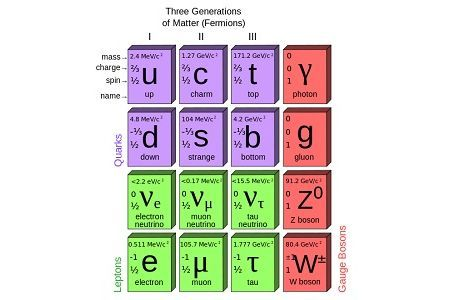
\includegraphics[clip=true, trim=0.0cm 0cm 0.0cm 0cm, width=1.0\textwidth]{figures/SM}\\
%      {Confirmed particles in the SM. Source: CERN
%        }
%      \label{fig:SM}
%  \end{center}
%\end{figure}

The quarks and gluons have color charge and interact through the strong force. There are three copies of each quark for each of the three different color charges.
The strength of the strong force increases with distance leading to color confinement where no free particles can exist with color charge.
Thus all quarks and gluons will form composite particles that are color neutral, called hadrons. There are two types of hadrons that have experimentally observed.
The first is a quark and an anti-quark referred to as a meson, such as a charged pion which is made of an up quark and a down antiquark.
The second is three quarks (or anti-quarks) referred to as a baryon, such as the proton and neutron.
Mesons and baryons can be either electrically charged or neutral.
Other combinations of quarks and gluons would be color neutral but have not been observed in nature.
One example is a pair of gluons that would always be electrically neutral.

When quarks and gluons are produced at high energies, the binding of the strong force normally results in numerous secondary quarks and antiquarks being produced.
These quarks and antiquarks will then form hadrons in a process called hadronization.
%form composite particles after being created at particle colliders like the LHC, they will normally create a large number of particles, called hadronization. 
All of the hadrons will be traveling in roughly the same direction resulting in a stream of collinear particles from the production point.
%The result is a large number of nearly colinear particles emanating from the interaction point. 
This beam of particles is referred to as a jet.

Most SM particles produced at the LHC, both fundamental and composite, have very short lifetimes preventing them from being directly detected. The only stable SM particles
at the LHC are the electron, proton, photon, and the neutrinos. Additionally, a free neutron has a lifetime of eight minutes but it may be stable inside a nucleus.
A few other particles have lifetimes long enough to be detected before decaying including the muon, pion, and kaon.

The proton-proton collisions at the LHC will create vast numbers of these SM particles. As the strong force has the largest coupling,
a large majority of the events will be the production of light quarks and gluons. A small fraction of the events (though a large total number given the very
high rate of collisions at the LHC) will produce particles such as $W$ and $Z$ bosons, top quarks, and the Higgs Boson.
These particles will quickly decay into other SM particles like muons, electrons, and b quarks. This production of stable and long lived SM particles,
particularly muons, form much of the background for the search for new heavy long-lived particles detailed in Chapter~\ref{sec:search}.

%\subsection{Cosmic rays \label{sec:cosmics}}
The production of SM particles proceeds not only in the proton-proton collisions at the LHC but also through astrophysical processes.
The earth is constantly being bombarded with high-momentum protons from astronomical sources. These protons interact with the earth's atmosphere
predominantly resulting in the production of numerous charged and neutral pions. Charged pions will then decay into high momentum muons.
As the muons will have a large relativistic boost, they will be able to reach the earth before decaying.
%At sea level the flux of muons is approximately one per 10$cm^2$.
Muons lose only a small amount of energy in interactions with matter,
allowing the highest-energy cosmic-ray muons to penetrate through large amounts of earth.
This allows cosmic-ray muons to pass through CMS creating another potential background for searches for new physics.

\section{Beyond Standard Model Theories and Heavy Stable Charged Particles \label{sec:BSM}}
More information about theories beyond the SM and heavy stable charged particles can be found in~\cite{Martin:1997ns, Tata:1997uf, Fairbairn:2006gg}.

While the SM has proven to be a very robust theory, there are reasons to believe it is not complete. These include runaway
radiative corrections to the Higgs mass and an inability to explain the astronomically observed dark matter~\cite{1983SciAm.248...96R}.
At a minimum, the theory must be replaced at the Planck energy scale ($1.22 \times 10^{19}$~GeV)
where the gravitational force becomes as strong as the other forces. To address issues like these numerous
theories have been put forth for physics beyond the SM (BSM). 
If these BSM theories are accurate, evidence of them could very well be present in the high energy collisions produced at the LHC.
Some of these BSM theories predict the existence of heavy meta-stable
charged particles (HSCP) with lifetimes greater than a few nanoseconds, long enough to traverse the length of typical particle detectors. 

One of the most popular BSM theories is supersymmetry (SUSY). A new symmetry is added that gives
each SM particle a superpartner particle with spin different by one half. The SUSY particles interact with the same coupling as their SM particles.
The names of the SUSY particles are generally found by prepending an s (for scalar) to the spin zero SUSY partners of spin 1/2 particles;
so the SUSY partner of the electron is the selectron. The names of other particles are found by adding --ino to the end of their names,
so the higgs SUSY partner is the higgsino.
As no SUSY particles have yet been discovered the
symmetry must be broken at some scale giving the SUSY particles masses larger than SM particles. In order to address the unresolved issues in the SM, this mass gap is
expected to be no larger than about 1 TeV. In addition to adding a new symmetry, most versions of SUSY have a new multiplicatively conserved quantity called R-parity
which is added to prevent rapid proton decay.
SUSY particles have an R-parity value of -1 while SM particles have a value of 1. This implies that the lightest SUSY particle (LSP) will be stable, and in most
SUSY theories it is taken to be electrically and color neutral so as to be the astronomically observed dark matter.

Other SUSY particles besides the LSP could have a long lifetime in certain areas of SUSY parameter space. In the minimal supersymmetric standard model (MSSM) the LSP is the
neutralino (superpartner of a neutrino) in most cases. The next lightest SUSY particle (NLSP) can be long-lived if the mass splitting between the NLSP and the LSP is small.
This can happen for various particles as the NLSP. 
For example, non-universal squark masses can be used to make the mass difference between the stop and the neutralino too small for the stop decay to a neutralino and
a bottom quark to be kinematically allowed.
%One case of interest is that of the scalar top (stop $\tilde{t}$) as the NLSP motivated by electroweak
%baryogenesis~\cite{Balazs:2004bu}. If the mass difference between the stop and the neutralino makes the stop decay to a neutralino and a b quark kinematically not
%allowed as arranged by non-universal squark masses, 
Then the stop decay happens via the radiative decay to a charm quark and neutralino, making the stop very long-lived.

Another variant of supersymmetry is split SUSY. In split SUSY, scalar SUSY particles have masses much larger than the other SUSY particles which are at the TeV scale.
The gluino $\tilde{g}$ (superpartner of the gluon) then decays through virtual squarks which 
is suppressed by a factor of $\tilde{m}^{-2}$, where $\tilde{m}$ is the mass of the squarks, allowing for the gluino to be quite long-lived.

Gluinos and stops have color charge and as such will form composite hadrons with SM quarks and gluons after production, referred to as $R$--hadrons.
These $R$--hadrons can be $R$--mesons, $R$--baryons, or, for gluinos, a glueball made of a gluino and a SM gluon.
%Examples of R-hadrons are shown in Fig.~\ref{fig:Composites}.
$R$--hadrons can be electrically neutral or have charge $Q$, taken in this paper unless otherwise stated as the absolute value of the charge,
of 1$e$ or 2$e$, where $e$ is the charge of the electron.
For gluinos, the fraction of gluinos forming glueballs, which are always electrically neutral, is
an unknown value in the theory. If the fraction is 100\%, then all gluino $R$--hadrons will be produced electrically neutral.
The mass spectrum of the $R$-hadrons is not well known.
If there are mass gaps between the $R$--hadrons larger than the pion mass, the heavier $R$--hadron would decay to the lighter $R$--hadron via the weak force.
It has historically been taken that all $R$--hadrons containing only gluons and up and down quarks are stable.
Recently, theories have been put forth~\cite{Mackeprang:2009ad} that only one $R$--baryon will be stable and the other $R$--baryons will immediately decay to it.
The fraction of $R$--hadrons emerging from the LHC collision point that are electrically charged would depend on the charge of that $R$--baryon.


%\begin{figure}
%  \begin{center}
%      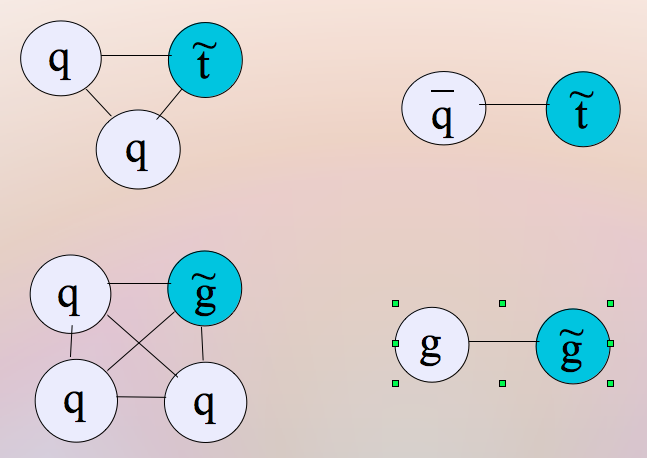
\includegraphics[clip=true, trim=0.0cm 0cm 0.0cm 0cm, width=1.0\textwidth]{figures/quarks}\\
%      {Different types of R-hadrons that color charged HSCP can form. Top left: Stop HSCP baryon with two SM quarks.
%Top right: Stop HSCP meson with a SM anti-quark. Bottom left: Gluino HSCP baryon with three SM quarks. Bottom right: Gluino HSCP glueball with a SM gluon.
%	}
%      \label{fig:Composites}
%  \end{center}
%\end{figure}

After the $R$--hadrons are produced at the LHC, they will propagate out to and interact with CMS.
In nuclear interactions with the detector, it is possible for the 
$R$--hadron to exchange quarks with the nucleons of the detector.
This can cause the
electrical charge of the $R$--hadron to change, possibly going from neutral
to charged or from charged to neutral. 

To cover all of the possible signatures that $R$--hadrons could have, two different modelings of nuclear interactions between $R$--hadrons and the CMS detector are considered.
The first is the model presented in~\cite{Kraan:2004tz, Mackeprang:2006gx}
which is referred to as the cloud model and results in a mixture of charged and neutral $R$--hadrons after a nuclear interaction.
The second model, referred to as charge-suppressed (CS), makes all $R$--hadrons neutral after a nuclear interaction.

For discovery at the LHC, the CS model is a somewhat more pessimistic model than the one discussed in~\cite{Mackeprang:2009ad}.
The model results in all $R$-hadrons becoming electrically neutral due to a combination of baryon exchange with the detector and the $R$-hadron mass spectrum.
$R$--mesons can interact with protons and neutrons in the detector converting into $R$--baryons and releasing a pion.
The reverse process is unlikely to occur due to the lack of pions in the detector material and limited phase space.
If the mass spectrum is as in~\cite{Mackeprang:2009ad}, then this would result in all $R$--hadrons becoming the charge of the lightest $R$--baryon in the model
after a few interactions. If this $R$--baryon is neutral, then essentially all $R$--hadrons will be neutral after passing through the calorimeter of CMS
(see Sec.~\ref{sec:subsystems}).

A third possible type of HSCP in SUSY is the production of long-lived staus $\tilde{\tau}$ in gauge mediated symmetry breaking (GMSB)~\cite{Giudice:1998bp}. 
In GMSB, the gravitino is very light and almost always the LSP.
GMSB models are characterized by six parameters which determine the mass hierarchy and decays of SUSY particles.
One of these parameters is the number N of SU(5) chiral multiplets added to the model which act as ``messengers''.
As long as N is not too small the NLSP is likely to be the stau.
%The lifetime of the stau is given by~\cite{Fairbairn:2006gg}
%\begin{equation}
%\tau_{Stau} = 0.1 \left(\frac{100 GeV}{m_{Stau}}\right)^5 \left(\frac{m_{\tilde{G}}}{2.4 eV}\right) mm/c
%\label{eq:lifetime}
%\end{equation}
%with $m_{\tilde{G}}$, the gravitino mass, set by
%\begin{equation}
%m_{\tilde{G}} = 2.4 c_{Grav} \left(\frac{\sqrt{M\Lambda}}{100 TeV}\right)^2 eV
%\label{eq:gravmass}
%\end{equation}
%with $\Lambda$ being the effective SUSY breaking scale, M the mass of the messengers, and
%$c_{Grav}$ the ratio between the fundamental SUSY breaking scale and the effective one felt by the messenger particles.
%The parameter $c_{Grav}$ relates to how the SUSY breaking is transmitted to the messengers, if the communication is done perturbatively then $c_{Grav}$
%will be very large giving the stau a long lifetime.
Another one of the parameters is $c_{Grav}$ which relates to how the SUSY breaking is transmitted to the messengers.
If the communication is done perturbatively, then $c_{Grav}$ will be very large.
The large value of $c_{Grav}$ results in the stau having a long lifetime.

Other BSM theories besides SUSY can also contain HSCPs.
An interesting scenario for HSCP is the production of particles with charge not equal to $1e$.
One model that includes non-unit charged HSCP is the production of particles that are neutral under $SU(3)_C$ and $SU(2)_L$ 
but have electric charge meaning they only couple to the photon and Z boson through $U(1)_Y$ interactions~\cite{Langacker:2011db}.
%The electric charge Q of the particle is not constrained to be 1e.
%Note here and for the rest of this paper Q is taken as the absolute value of the electrical charge unless specifically stated otherwise.
The HSCP could be produced with fractional charge ($<1e$) or multiple charge ($>1e$).

%Another BSM theory that includes HSCP is Universal Extra Dimensions (UED). In UED SM fields, quarks, and gluons propagate through new dimensions with the
%known SM fields representing the ground state mode in the new dimensions. States in excited modes in the new dimension would be seen as new particles.
%A new quantum number is introduced in UED for momentum conservation in the extra dimensions that forces the lightest excited particle to be stable,
%making it a dark matter. The excited states of light SM particles could have long enough lifetimes to be experimentally detectable.

